\chapter*{2 Versuchsdurchführung und Auswertung}
\addcontentsline{toc}{chapter}{2 Versuchsdurchführung und Auswertung}
\setcounter{chapter}{2}
\setcounter{section}{0}
\setcounter{subsection}{0}
 
    \section{Versuch 1 - Bestimmung der Viskosität von Getriebeöl mit der Kugelfallmethode}
    \label{sec:Versuch1}
        
        \subsection{Aufbau \& Durchführung}

            \begin{figure}[H]
                \centering
                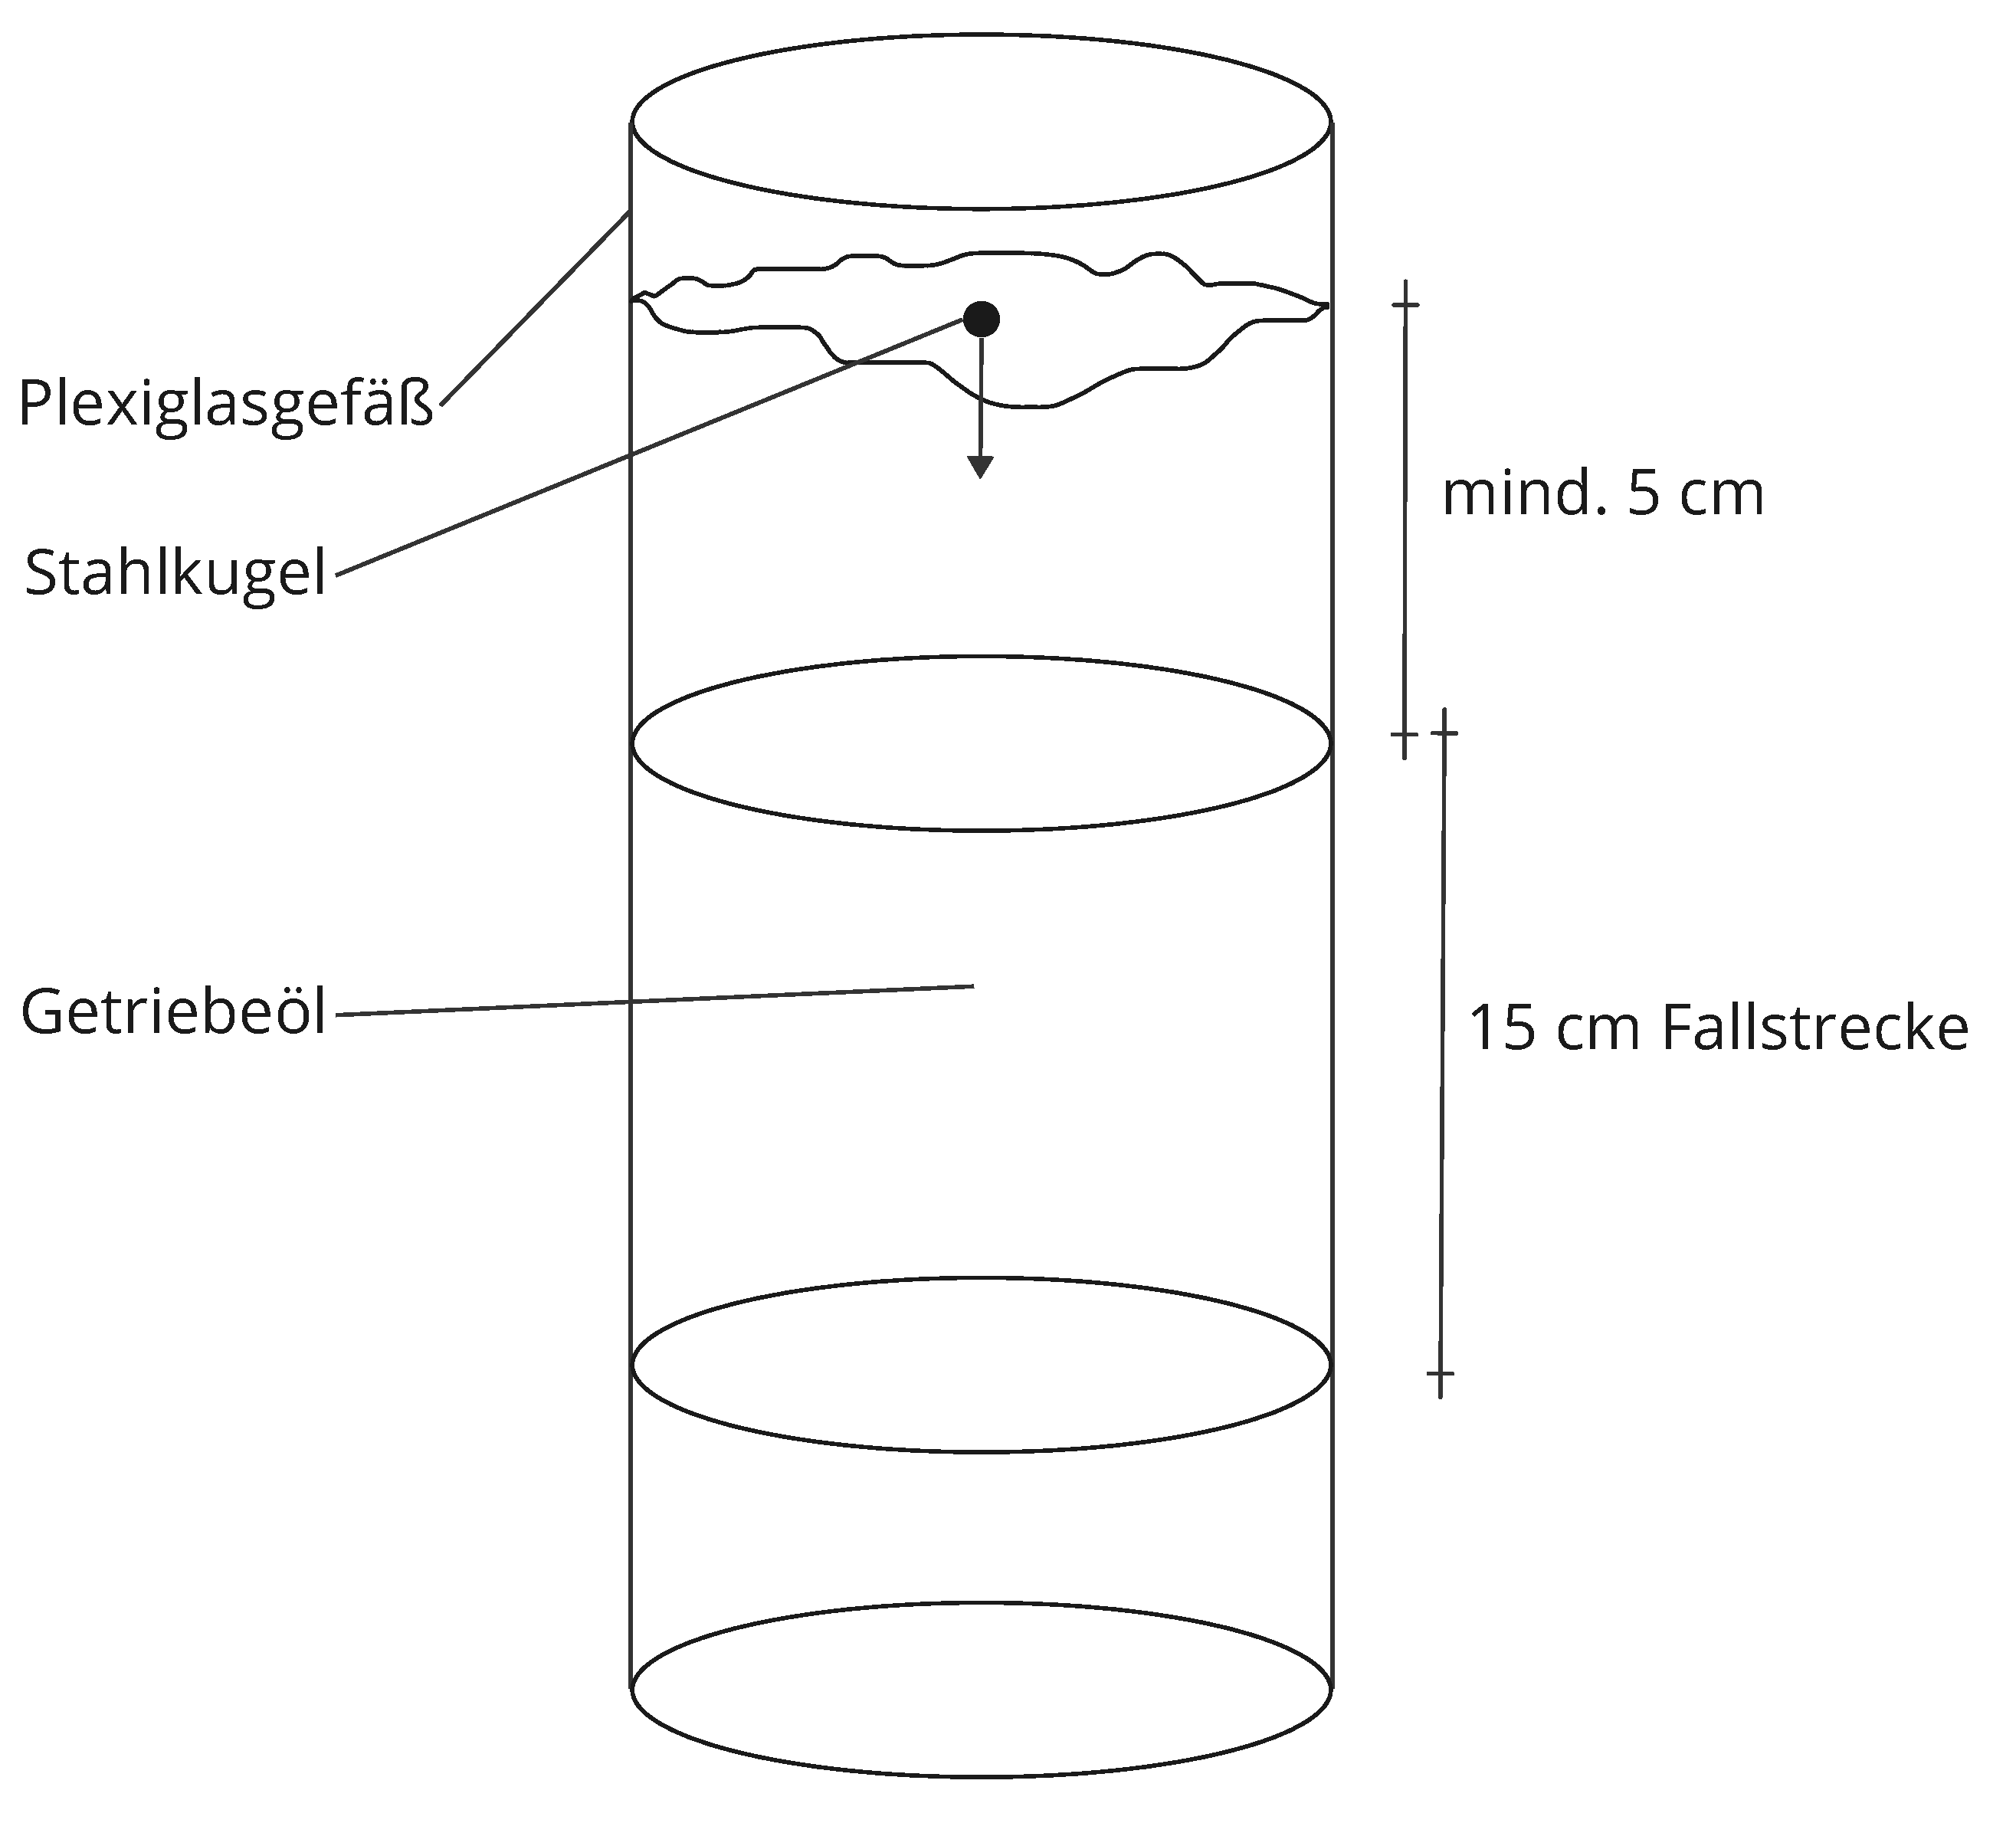
\includegraphics[width=0.5\textwidth]{bilder/AufbauV1.pdf}
                \caption{Aufbau des Versuchs 1.}
                \label{fig:AufbauV1}
            \end{figure}

            In Versuch 1 wird die dynamische Viskosität von Getriebeöl mit Hilfe der Kugelfallmethode bestimmt. Der Versuchsaufbau sieht wie folgt aus (siehe Abb~\ref{fig:AufbauV1}):
            Ein Plexiglaszylinder, welcher mind. $30\ \mathrm{cm}$ hoch ist, wird mit Getriebeöl OKS 3740 befüllt. Nun wird eine Fallstrecke $L$ von $15\ \mathrm{cm}$ markiert. Diese hat mind. $5\ \mathrm{cm}$ Abstand zur Öffnung des Gefäßes. Anschließend werden jeweils 10 Kugeln (V2A-Stahl) in der Mitte des Gefäßes fallen gelassen und die Fallzeit im Abschnitt $L$ gemessen. Dies wird für die Kugeldurchmesser $d = 1, 2, 3\ \mathrm{mm}$ und $4\ \mathrm{mm}$ wiederholt. Die $3\ \mathrm{mm}$-Kugel wird 30 Mal gemessen und später eine Verteilung zufällig verteilter Messwerte graphisch darzustellen.
            Die Viskosität lässt sich dann über die Formel~\ref{eq:dynamischeViskosität} der dynamischen Viskosität $\eta$ berechnen, oder mit Hilfe eines Graphens.

            Für die statistische Auswertung der Messwerte wird die Software Origin verwendet. Es wird eine Häufigkeitsverteilung der Messwerte erstellt und eine Gaußkurve angepasst.

        \subsection{Auswertung}

            \subsubsection{a)}

            Zunächst wurde der Durchmesser $d$ stichprobenartig von $3$ Kugeln gemessen (siehe Tabelle~\ref{tab:MesswerteDurchmesser}):

            \begin{table}[H]
                \centering
                \caption{Ergebnis der Messung der Kugeldurchmesser.}
                \vspace*{.5em}
                \begin{tabular}{|l||r||r|r|r|}
                    \hline
                    & $d_{1}$ & $d_{2}$ & $d_{3}$ & $d_{4}$\\
                    \hline \hline
                    Mittelwert $[\mathrm{mm}]$ & $0.993$ & $1.997$ & $2.99$ & $3.99$\\
                    Standartabweichung $[\mathrm{mm}]$ & $0.00577$ & $0.00577$ & $0.00000$ & $0.00577$\\
                    Mittelwert der Standardabweichung $[\mathrm{mm}]$ & $0.00333$ & $0.00333$ & $0.00000$ & $0.00333$\\
                    \hline
                \end{tabular}
                \label{tab:MesswerteDurchmesser}
            \end{table}

            Danach wurden die Fallzeiten $t_{i}$ der Kugeln gemessen (siehe Tabelle~\ref{tab:MesswerteFallzeiten}):

            \begin{table}[H]
                \centering
                \caption{Ergebnis der Messung der Fallzeiten.}
                \vspace*{.5em}
                \begin{tabular}{|l||r|r|r|r|}
                    \hline
                    $n$ & $t_{1}$ & $t_{2}$ & $t_{3}$ & $t_{4}$\\
                    \hline \hline
                    1 & 79,23    & 20,17    & 9,28    & 5,28\\
                    2 & 79,47    & 20,47    & 9,25    & 5,31\\
                    3 & 79,88    & 20,22    & 9,14    & 5,38\\
                    4 & 79,07    & 20,49    & 9,25    & 5,39\\
                    5 & 79,66    & 20,58    & 9,28    & 5,31\\
                    6 & 79,07    & 20,06    & 9,25    & 5,43\\
                    7 & 79,35    & 20,11    & 9,08    & 5,41\\
                    8 & 78,42    & 20,21    & 9,28    & 5,41\\
                    9 & 76,95    & 20,19    & 9,29    & 5,23\\
                    10 & 79,36   & 19,60    & 9,34    & 5,40\\
                    11 &         &          & 9,27    &     \\
                    12 &         &          & 9,10    &     \\
                    13 &         &          & 9,24    &     \\
                    14 &         &          & 9,25    &     \\
                    15 &         &          & 9,17    &     \\
                    16 &         &          & 9,26    &     \\
                    17 &         &          & 9,14    &     \\
                    18 &         &          & 9,30    &     \\
                    19 &         &          & 9,19    &     \\
                    20 &         &          & 9,29    &     \\
                    21 &         &          & 9,79    &     \\
                    22 &         &          & 9,20    &     \\
                    23 &         &          & 9,16    &     \\
                    24 &         &          & 9,19    &     \\
                    25 &         &          & 9,01    &     \\
                    26 &         &          & 9,10    &     \\
                    27 &         &          & 9,22    &     \\
                    28 &         &          & 9,20    &     \\
                    29 &         &          & 9,05    &     \\
                    30 &         &          & 9,14    &     \\
                    \hline
                    Mittelwert $[s]$ & 79,00 & 20,20 & 9,20 & 5,36\\
                    Standardabweichung $[s]$ & 0,83423 & 0,27681 & 0,13433 & 0,06737\\
                    Mittelwert der Standardabweichung $[s]$ & 0,26381 & 0,08753 & 0,02453 & 0,02130\\
                    \hline
                \end{tabular}
                \label{tab:MesswerteFallzeiten}
            \end{table}

            Die Länge $L$ der Fallstrecke beträgt $15\ \mathrm{cm}$. Die Dichte der Kugeln (V2A-Stahl) $\rho_{\mathrm{K}}$ und die Dichte des Getriebeöls OKS 3740 $\rho_{\mathrm{F}}$ betragen:

            \begin{align}
                \rho_{\mathrm{K}} &= 7900\ \mathrm{\frac{kg}{m^{3}}}\\
                \rho_{\mathrm{F}} &= 850\ \mathrm{\frac{kg}{m^{3}}}
            \end{align}

            Somit lassen sich mit der Formel für die dynamische Viskosität $\eta$:

            \begin{equation}
                \eta = \frac{(\rho_{\mathrm{K}} - \rho_{\mathrm{F}}) \cdot g}{18 \cdot L} \cdot d^{2} \cdot t
                \label{eq:dynamischeViskosität}
            \end{equation}

            die Viskosität $\eta$ der Flüssigkeit berechnen. Die Fallbeschleunigung $g$ beträgt $9,81\ \mathrm{\frac{m}{s^{2}}}$. Die Ergebnisse sind in Tabelle~\ref{tab:ErgebnisseDynViskosität} zu sehen.

            \begin{table}[H]
                \centering
                \caption{Ergebnis der Berechnung der dynamischen Viskosität.}
                \vspace*{.5em}
                \begin{tabular}{|l||r|r|r|r|}
                    \hline
                    & $d_{1}$ & $d_{2}$ & $d_{3}$ & $d_{4}$\\
                    \hline \hline
                    Viskosität $[\mathrm{Pa \cdot s}]$ & $1.99502$ & $2.06089$ & $2.10923$ & $2.18428$\\
                    \hline
                \end{tabular}
                \label{tab:ErgebnisseDynViskosität}
            \end{table}

            Für die Größtfehlerabschätzung werden folgende Werte verwendet (siehe Tabelle~\ref{tab:Fehlerabschaetzung}):

            \begin{table}[H]
                \centering
                \caption{Fehlerabschätzung der Messwerte.}
                \vspace*{.5em}
                \begin{tabular}{|l||r|}
                    \hline
                    $\Delta L [\mathrm{mm}]$ & 5.00\\
                    \hline
                    $\Delta d [\mathrm{mm}]$ & 0.01\\
                    \hline
                    $\Delta t [\mathrm{s}]$ & 0.4\\
                    \hline
                \end{tabular}
                \label{tab:Fehlerabschaetzung}
            \end{table}

            Der Wert $0.4$ ergibt sich aus der zweifachen Reaktionszeit des Menschen.

            Mit diesen Werten lässt sich nun das folgende Ergebnis berechnen (siehe Tabelle~\ref{tab:Groesstfehler}):

            \begin{table}[H]
                \centering
                \caption{Größtfehlerberechnung (komponentenweise).}
                \vspace*{.5em}
                \begin{tabular}{|l||r|r|r|r|}
                    \hline
                    & $d_{1}$ & $d_{2}$ & $d_{3}$ & $d_{4}$\\
                    \hline \hline
                    Viskosität $[\mathrm{Pa \cdot s}]$ & $1.99502$ & $2.06089$ & $2.10923$ & $2.18428$\\
                    \hline
                    $\frac{\Delta L}{L}$ & $0.03333$ & $0.03333$ & $0.03333$ & $0.03333$\\
                    $\frac{\Delta d}{d}$ & $0.02013$ & $0.01002$ & $0.00669$ & $0.00501$\\
                    $\frac{\Delta t}{t}$ & $0.00506$ & $0.01979$ & $0.04337$ & $0.07470$\\
                    \hline
                    Größtfehler $[\mathrm{Pa \cdot s}]$ & $0.11676$ & $0.13013$ & $0.17589$ & $0.24691$\\
                    \hline
                \end{tabular}
                \label{tab:Groesstfehler}
            \end{table}

            Der Mittelwert der Viskosität beträgt somit: $\eta = 2.1 \pm 0.167\ \mathrm{Pa \cdot s}$.  Der Wert $0.167$ ist der Mittelwert der Größtfehler.

            Trägt man die Mittelwerte der Fallzeiten über $\frac{1}{d^{2}}$ in einem Graphen (\ref{fig:graph_01}) auf und lässt sich die Steigung berechnen, so erhält man eine zweite Möglichkeit die Viskosität zu berechnen. Die Steigung $m$ der Gerade entspricht in unserem Fall dem Wert: $78.219$. Die Viskosität $\eta$ lässt sich dann mit der Formel: 

            \begin{equation}
                \eta = \frac{m \cdot (\rho_{\mathrm{K}} - \rho_{\mathrm{F}}) \cdot g}{18 \cdot L}
            \end{equation}

            bestimmen. Das Ergebnis lautet: $\eta = 2.0 \pm 0.167\ \mathrm{Pa \cdot s}$. Hier wurde ebenfalls der Mittelwert der Größtfehler verwendet aus Tabelle~\ref{tab:Groesstfehler}.

            \begin{figure}
                \centering
                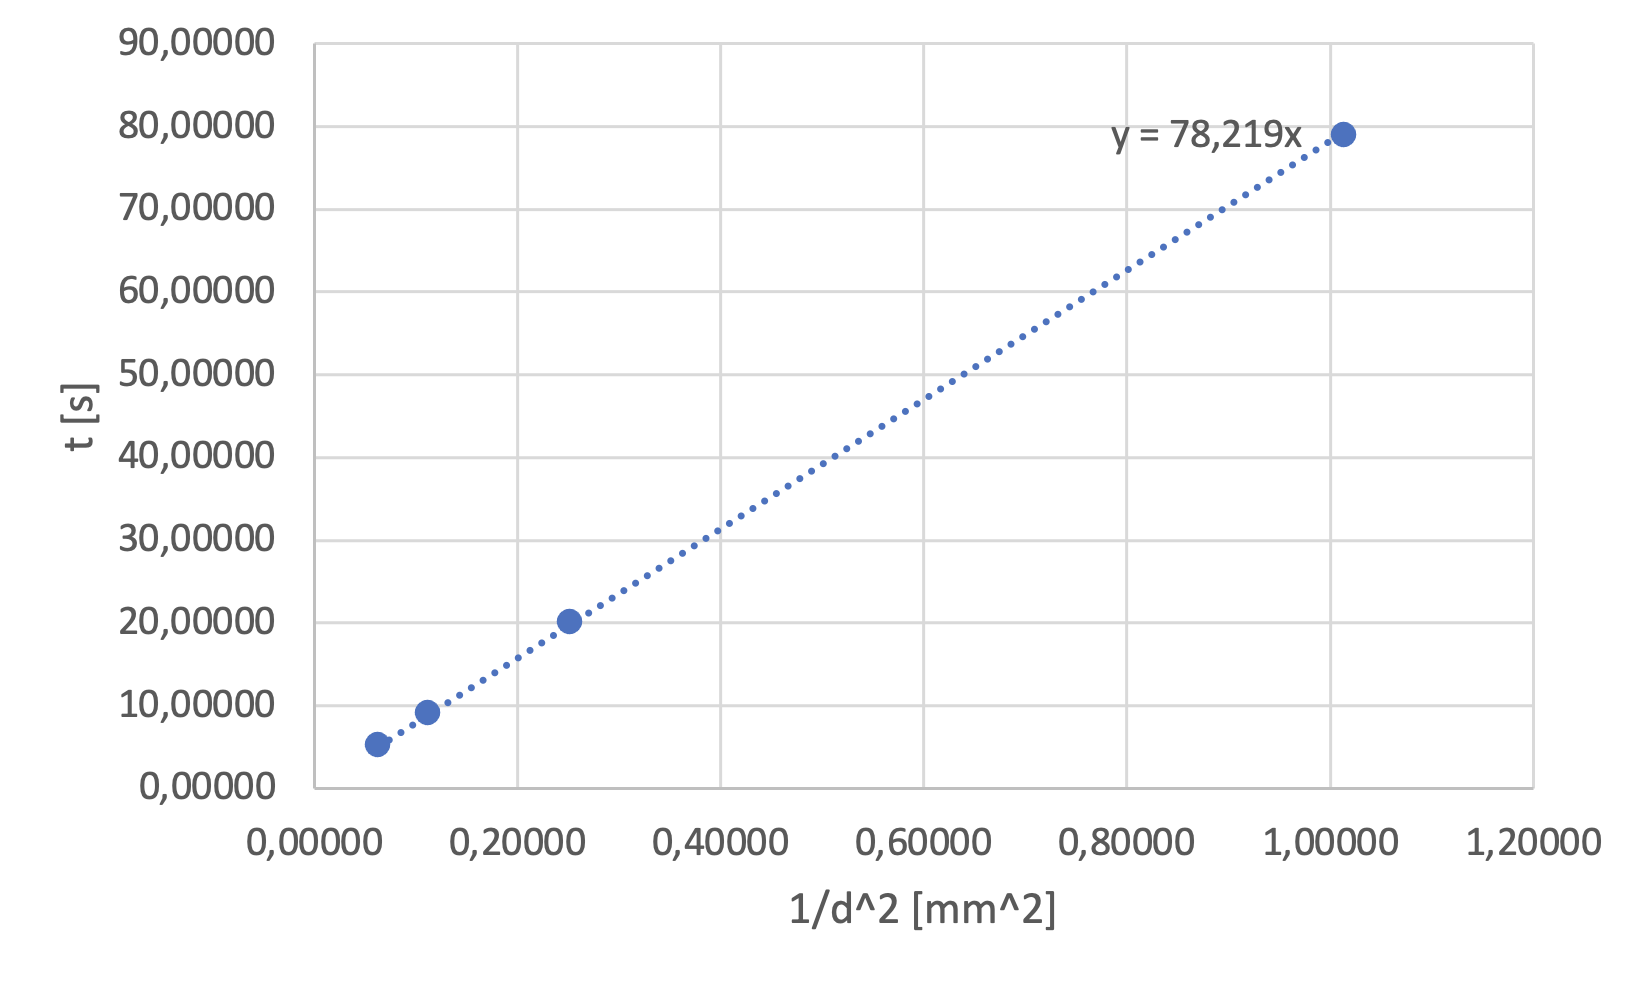
\includegraphics[width=0.8\textwidth]{bilder/Diagram_01.png}
                \caption{Fallzeiten über $\frac{1}{d^{2}}$.}
                \label{fig:graph_01}
            \end{figure}

            \subsubsection{b)}

            \begin{figure}[H]
                \centering
                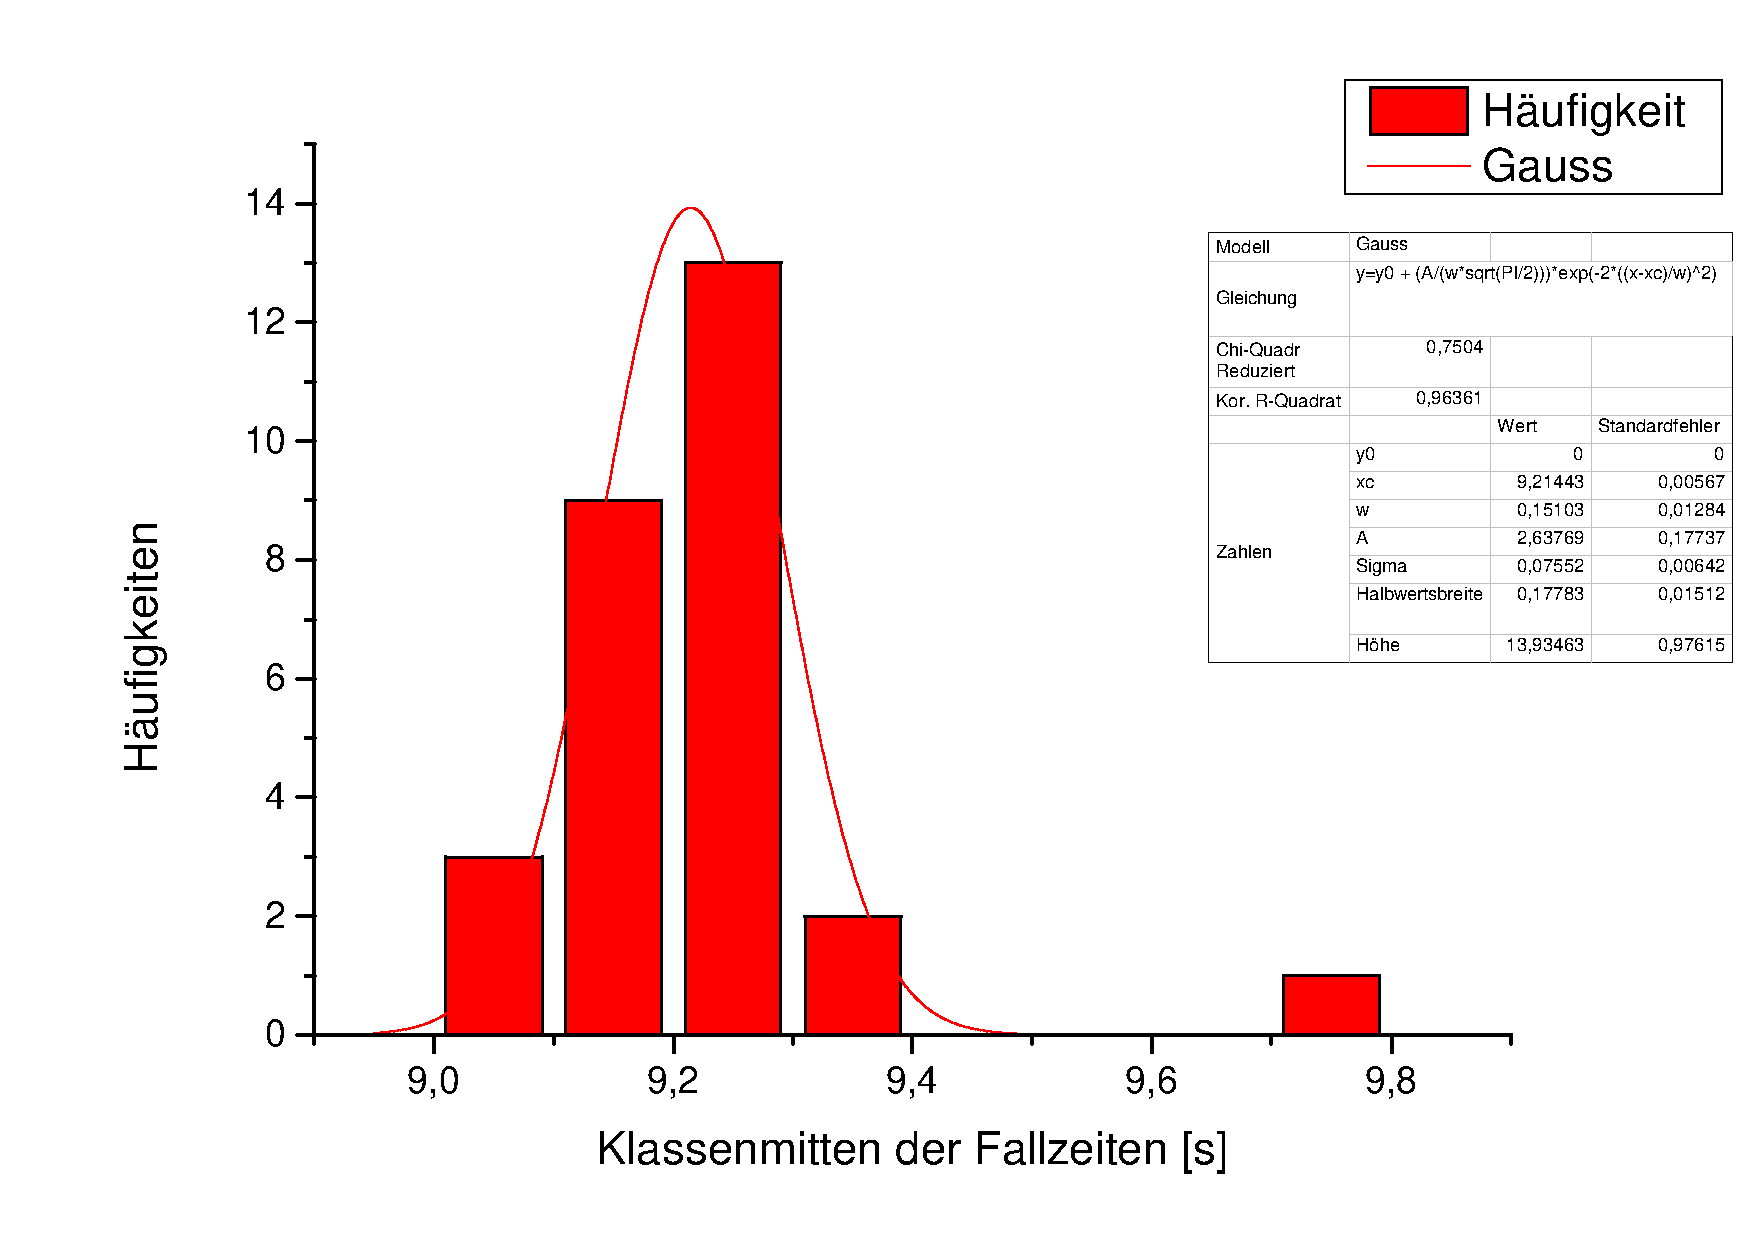
\includegraphics[width=0.8\textwidth]{bilder/Diagramm Fallzeiten.pdf}
                \caption{Häufigkeitsverteilung der Fallzeiten der $3\ \mathrm{mm}$-Kugel.}
                \label{fig:graph_02}
            \end{figure}

            Die Abbildung~\ref{fig:graph_02} zeigt die Häufigkeitsverteilung der einzelnen Messwerte der Fallzeiten der $3\ \mathrm{mm}$-Kugel. Die dünne rote Linie im Hintergrund stellt die Gaußkurve dar, welche mit einem Fit an die Messwerte angepasst wurde.

            Aus dem Diagram lässt sich anhand des Wertes xc der Mittelwert der Fallzeiten ablesen. Dieser beträgt hier $9.21443\ \mathrm{s}$ und ist damit minimal höher als der Mittelwert der Fallzeiten aus Tabelle~\ref{tab:MesswerteFallzeiten}. Zudem lässt sich anhand des Wertes Sigma die Standardabweichung der Messwerte ablesen. Dieser beträgt hier $0.07552\ \mathrm{s}$ und ist damit viel geringer als der Mittelwert der Standardabweichung aus Tabelle~\ref{tab:MesswerteFallzeiten}. Woran das liegt ist uns nicht klar.

        \subsection{Diskussion}

            Zu den Messwerten der Fallzeiten lässt sich nicht viel sagen. Sie liegen alle in einem angemessenem Zeitraum und auch die Standardabweichung ist gering. Die Werte der Fallzeiten in Graph~\ref{fig:graph_01} veranschaulichen einigermaßen gut, dass sich die Werte in einem normalen Bereich befinden.

            Betrachten wir nun die berechnete Viskosität, so fällt auf, dass die Viskosität kontinuierlich bei steigendem Kugeldurchmesser zunimmt. Dies ist zu erwarten, da bei steigendem Durchmesser (und Masse) die Fallgeschwindigkeit zunimmt und somit weniger laminare Strömung und mehr Turbulenz entsteht. Turbulenz benötigt Energie, wodurch die Geschwindigkeit der Kugel fällt, was zu einer höheren Viskosität führt.

            Im Vergleich dazu betrachten wir nun den Wert, welcher durch die Steigung der Gerade aus Graph~\ref{fig:graph_02} berechnet wurde. Hier wurde eine gerade durch die 4 Fallzeiten der Kugeln gelegt. Allerdings wurden diese Werte über $\frac{1}{d^{2}}$ gemappt, was dazu führt, dass die kleineren Durchmesser, vor allem die $1\ \mathrm{mm}$-Kugel, einen größeren Einfluss auf die Steigung haben, als die größeren Kugeln. Schauen wir uns den berechneten Wert der Viskosität an, so sehen wir, dass dieser um einiges geringer ist, als der berechnete Wert aus der ersten Methode. Zudem sehen wir, dass er sehr nah am Wert der $1\ \mathrm{mm}$-Kugel liegt.

            Allerdings ist der Wert immer noch höher als der Literaturwert. Dies kann daran liegen, dass zwar unserer Lufttemperatur $20\ \mathrm{^\circ C}$ betrug, die Temperatur der Flüssigkeit aber nicht. Zudem kann es auch sein, dass die Kugeln nicht perfekt rund sind, was zu einer höheren Reibung führt. Andere Messfehler fließen auch mit ein.
        
    \section{Versuch 2 - Bestimmung der Glycerinkonzentration mit dem Kapillarviskosimeter}
    \label{sec:Versuch2}

        \subsection{Aufbau \& Durchführung}
            
            In Versuch 2 wird die kinematische Viskosität $\nu$ einer Glycerin-Wasser-Mischung mit Hilfe eines Kapillarviskosimeters bestimmt. Der Versuchsaufbau sieht wie folgt aus (siehe Abbildung \ref{fig:Kapillarviskosimeter}).

            \begin{figure}[h]
                \centering
                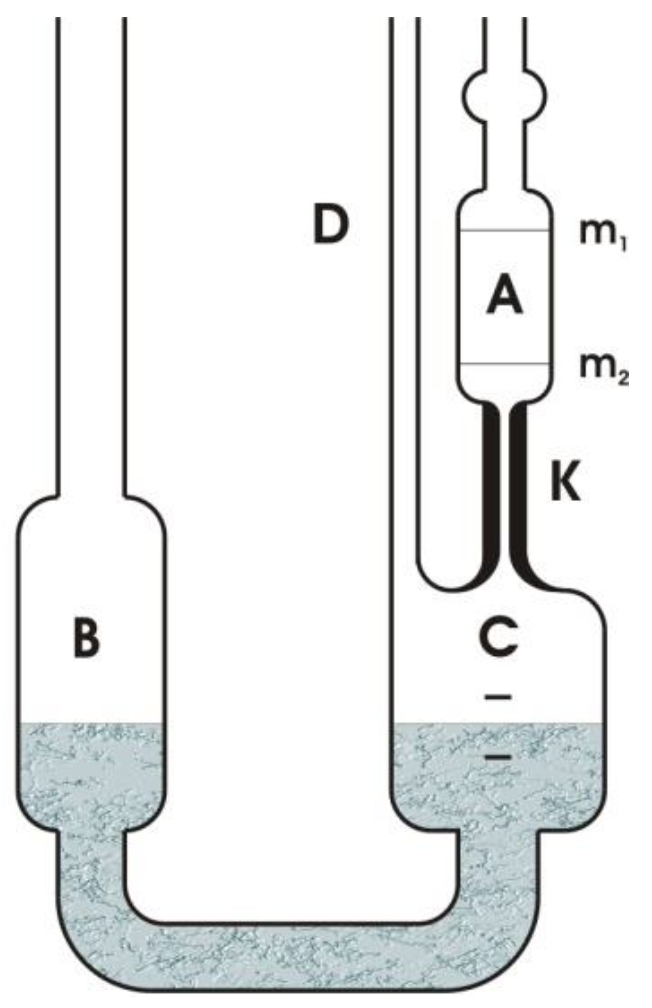
\includegraphics[width=0.5\textwidth]{bilder/Kapillarviskosimeter.png}
                \caption{Aufbau des Kapillarviskosimeters.}
                \label{fig:Kapillarviskosimeter}
            \end{figure}

            Ein Wassertank ist mit Wasser befüllt und wird auf konstante $30\ \mathrm{^\circ C}$ erwärmt. In diesen Wassertank wird das Kapillarviskosimeter eingetaucht. Ein genauerer Aufbau des Kapillarviskosimeters ist in Abbildung~\ref{fig:Kapillarviskosimeter} zu sehen. Dieses Funktioniert so, dass die Öffnung D zugehalten wird, die Flüssigkeit durch Ansaugen an Öffnung A, nach oben gesaugt wird, bis die Flüssigkeit den Raum A komplett ausfüllt, sodass die Flüssigkeit zwischen $m_1$ und $m_2$ vorhanden ist. Danach wird die Öffnung an D geöffnet und auch an A. Dann wird die Zeit gemssen, die die Flüssigkeit benötigt um die Strecke zwischen $m_{1}$ und $m_{2}$ abzusinken. Mit den Messwerten und der Formel

            \begin{equation}
                \nu = K \cdot t
                \label{eq:kinetamischeViskosität}
            \end{equation}

            lässt sich die kinematische Viskosität berechnen. Dabei ist $K$ eine Konstante, die für jedes Kapillarviskosimeter unterschiedlich ist. Diese Werte sind allerdings schon vorgegeben. Zum Schluss soll das Gesetz von Hagen-Poiseuille überprüft werden. Es wird geschaut, ob die Potenz aus unseren Werten die gleiche ist, wie die Potenz aus dem Gesetz von Hagen-Poiseuille.

        \subsection{Auswertung}

            Die folgende Tabelle~\ref{tab:MesswerteKapillarviskosimeter} enthält alle Messwerte von zwei verschiedenen Kapillarviskosimetern. Es handelt sich dabei um Typ III und IIc.

            \begin{table}[H]
                \centering
                \caption{Messwerte der Fallzeiten.}
                \vspace*{.5em}
                \begin{tabular}{|l||r|r|}
                    \hline
                    & Typ III & Typ IIc\\
                    \hline\hline
                    Fallzeit $t_{1}\ [\mathrm{s}]$ & $66.04$ & $414.74$\\
                    Fallzeit $t_{2}\ [\mathrm{s}]$ & $64.80$ & $415.32$\\
                    Fallzeit $t_{3}\ [\mathrm{s}]$ & $65.08$ & $414.39$\\
                    \hline
                    Mittelwert $t\ [\mathrm{s}]$ & $65.30$ & $414.80$\\
                    Standardabweichung $[\mathrm{s}]$ & $0.65033$ & $0.46972$\\
                    \hline
                    K $\mathrm{[mm^{2}/s^{2}]}$ & $0.93419$ & $0.29979$\\
                    \hline
                \end{tabular}
                \label{tab:MesswerteKapillarviskosimeter}
            \end{table}

            Die kinematische Viskosität lässt sich nun mit Hilfe der Formel~\ref{eq:kinetamischeViskosität} berechnen (siehe Tabelle~\ref{tab:ErgebnisseKapillarviskosimeter}):

            \begin{table}[H]
                \centering
                \caption{Ergebnisse der kinematischen Viskosität.}
                \vspace*{.5em}
                \begin{tabular}{|l||r|r|}
                    \hline
                    & Typ III & Typ IIc\\
                    \hline\hline
                    $\nu\ [\mathrm{mm^{2}/s}]$ & $61.00296$ & $124.35789$\\
                    \hline
                \end{tabular}
                \label{tab:ErgebnisseKapillarviskosimeter}
            \end{table}

            Nun soll das Gesetz von Hagen-Poiseuille überprüft werden. Dazu wird die Formel

            \begin{equation}
                \log\left(\frac{\Delta t_{2}}{\Delta t_{1}}\right) = x \cdot \log\left(\frac{R_{1}}{R_{2}}\right)
                \label{eq:x-Formel}
            \end{equation}

            verwendet. Wobei $R$ der Innendurchmesser der Kapillare ist. $R_{1} = 1.005\ \mathrm{mm}$ und $R_{2} = 0.75\ \mathrm{mm}$. Die Werte $\Delta t$ sind die Mittelwerte der Fallzeiten.

            Stellt man die Formel~\ref{eq:x-Formel} nun nach $x$ um und setzt die berechneten Werte ein erhalten wir:

            $$x = 6.31682$$

            $x$ stellt die Potenz aus dem Gesetz von Hagen-Poiseuille dar. Diese sollte im Idealfall $4$ betragen.

            Um nun final die Konzentration von Glycerin in der Glycerin-Wasser-Mischung zu bestimmen, benutzten wir die Werte aus dem Anhang und erstellen uns einen Graph, an dem wir die Konzentration ablesen können. Dieser ist in Abbildung~\ref{fig:GraphKonzentration} zu sehen.

            \begin{figure}[H]
                \centering
                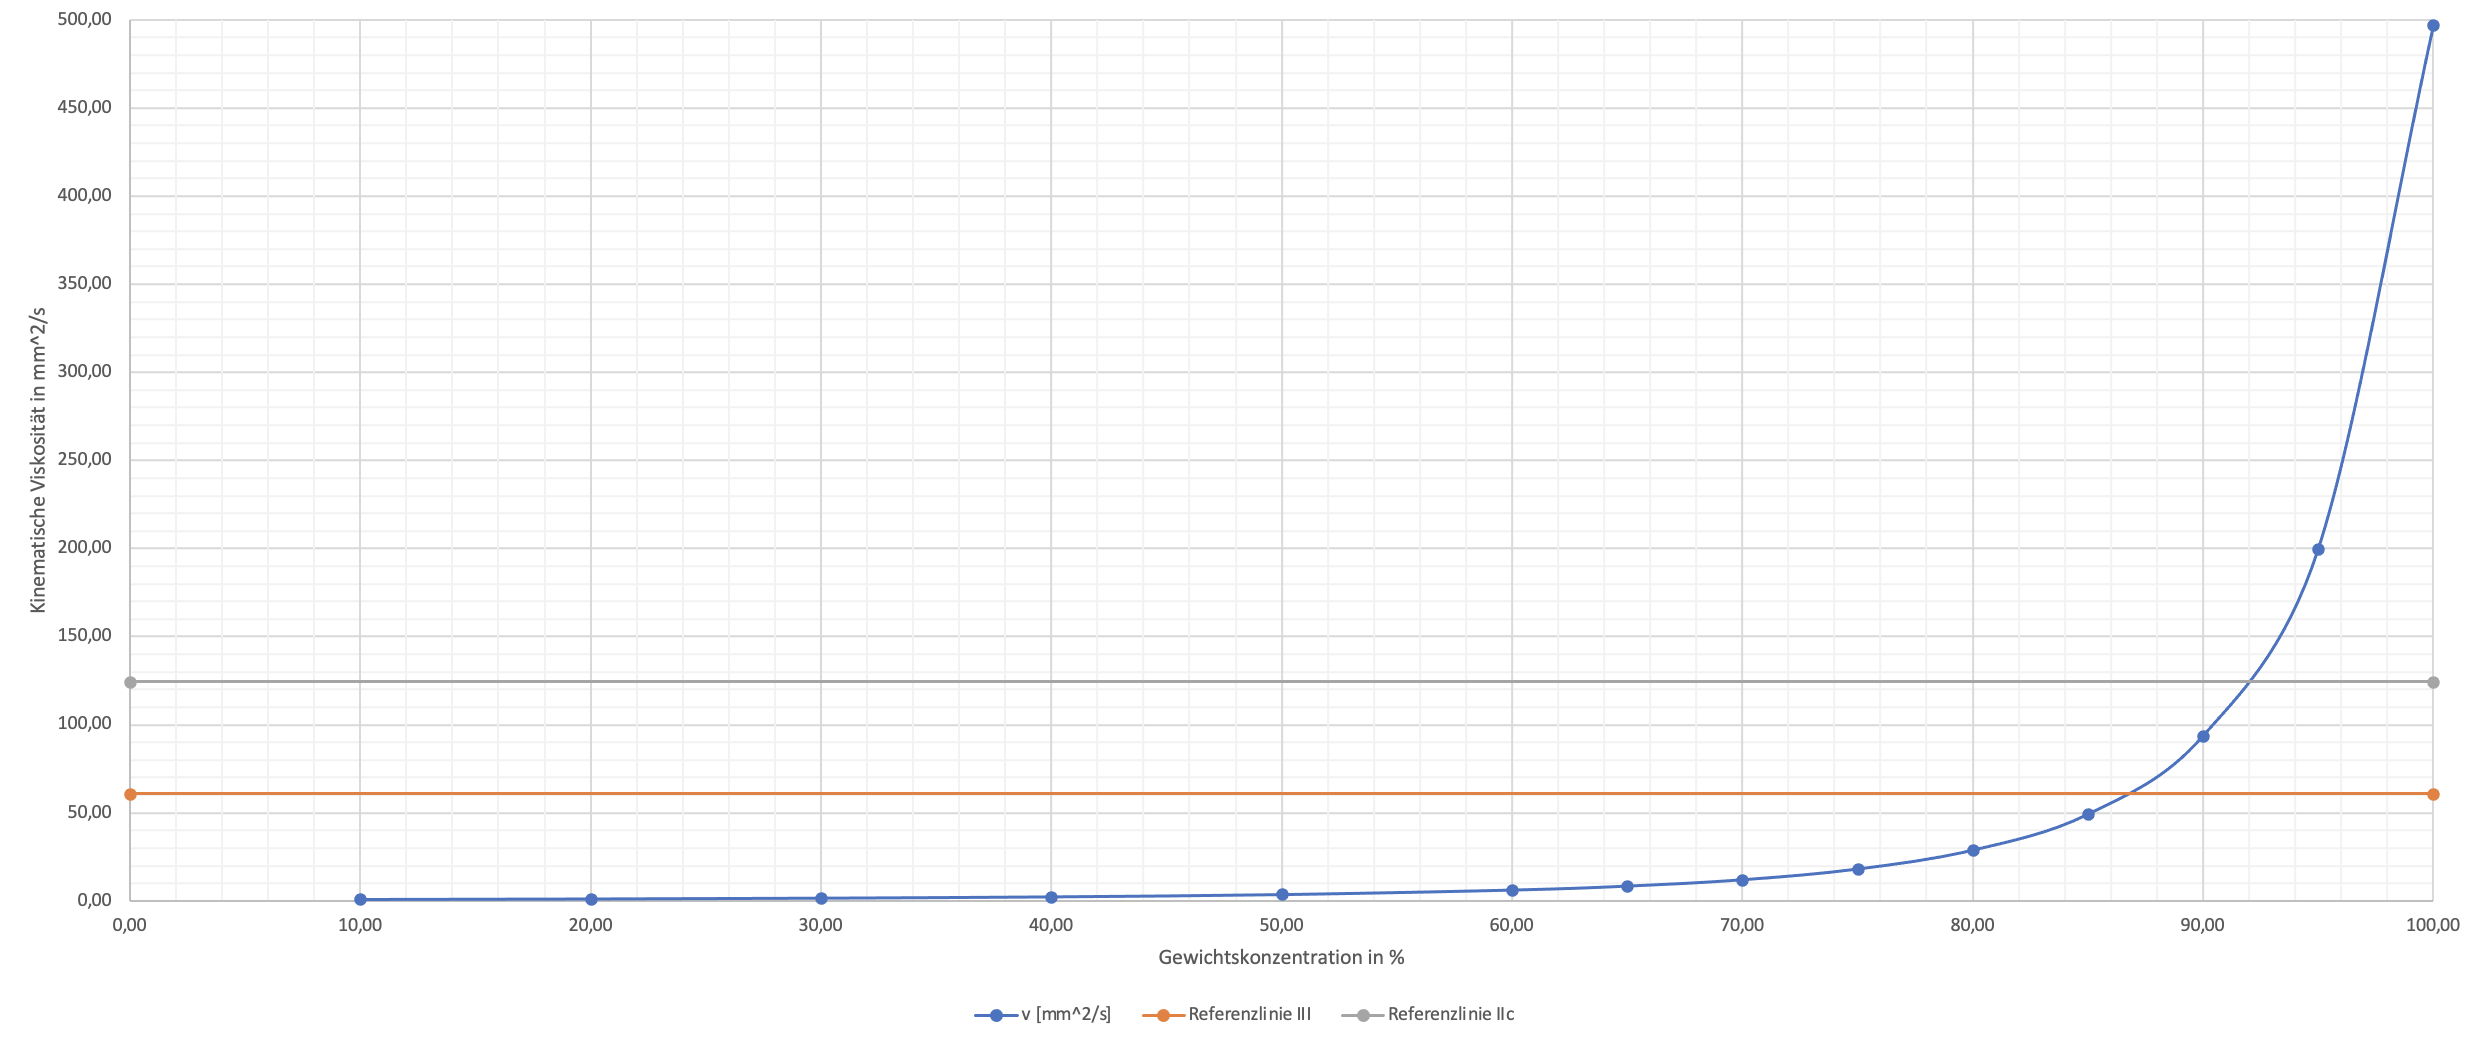
\includegraphics[width=0.8\textwidth]{bilder/Konzentration.png}
                \caption{Graph zur Bestimmung der Glycerinkonzentration.}
                \label{fig:GraphKonzentration}
            \end{figure}

            Lesen wir nun die Konzentration der Flüssigkeiten ab, so erhalten wir (siehe Tabelle~\ref{tab:Konzentration}):

            \begin{table}[H]
                \centering
                \caption{Konzentration der Flüssigkeiten.}
                \vspace*{.5em}
                \begin{tabular}{|l||r|r|}
                    \hline
                    & Typ III & Typ IIc\\
                    \hline\hline
                    Glycerinkonzentration $[\mathrm{\%}]$ & $78$ & $92$\\
                    \hline
                \end{tabular}
                \label{tab:Konzentration}
            \end{table}

        \subsection{Diskussion}

            Zu den Fallzeiten der Flüssigkeiten gibt es nicht viel zu sagen. Die Werte $66.04\ \mathrm{s}, 64.80\ \mathrm{s}, 65.08\ \mathrm{s}$ und $414.74\ \mathrm{s}, 415.32\ \mathrm{s}$, $414.39\ \mathrm{s}$ liegen alle in einem angemessenen Rahmen und auch die Standardabweichung von $0.65033\ \mathrm{s}$ und $0.29979\ \mathrm{s}$ ist gering. Es war zudem auch zu erwarten, dass die Fallzeiten von Typ IIc um einiges höher sind, als die von Typ III. Dies liegt daran, dass die Kapillare von Typ IIc einen kleineren Innendurchmesser hat, als die von Typ III. Wenn wir nun die kinematische Viskosität berechnen, so sehen wir allerdings, dass der Wert der Flüssigkeit von Typ IIc das doppelte von Typ III beträgt, nämlich $124.35789\ \mathrm{\frac{mm^2}{2}}$ im Vergleich zu $61.00296\ \mathrm{\frac{mm^2}{2}}$. Dies kann daran liegen, dass sich in diesem Gefäß eine frischere Lösung befindet, als in dem anderen Gefäß. Dies kommt davon, dass Glycerin hygroskopisch ist und verwässert und dementsprechend ausgetauscht werden muss.

            Diese Werte haben nun auch eine Auswirkung auf die Überprüfung des Gesetzes von Hagen-Poiseuille. Der Wert $x$ ist mit $6.31682$ deutlich höher, als der erwartete Wert $4$. Dies kommt davon, dass die Viskositäten der beiden Flüssigkeiten nicht identisch sind, sondern extrem unterschiedliche Werte betragen.